% Chapter 1
\chapter{General Introduction} % Main chapter title
%\addchap[]{General Introduction}
\label{Intro} % For referencing the chapter elsewhere, use \ref{Chapter1} 
%----------------------------------------------------------------------------------------

% Define some commands to keep the formatting separated from the content 
\newcommand{\keyword}[1]{\textbf{#1}}
\newcommand{\tabhead}[1]{\textbf{#1}}
\newcommand{\code}[1]{\texttt{#1}}
\newcommand{\file}[1]{\texttt{\bfseries#1}}
\newcommand{\option}[1]{\texttt{\itshape#1}}
\newcommand{\krilllatin}{\textit{Euphausia superba}}
\newcommand{\krilllatinshort}{\textit{E. superba}}
%----------------------------------------------------------------------------------------

In this section, I would like to introduce the scientific background for this
dissertation which studied seasonal, physiological and genetic functions in
Antarctic krill, \textit{Euphausia superba}, under different latitudinal light
regimes. First, I will explain the importance of \textit{E. superba} in the
Southern Ocean ecosystem, the impact of fisheries, as well as the effects of
climate change and potential phenological mismatches on this species.
Afterwards, I will summarize findings from field studies that show that
Antarctic krill has evolved pronounced seasonal cycles of physiology and
behaviour to adapt to the highly variable environment in the Southern Ocean.
Then, I will integrate information about the seasonal timing system in
Antarctic krill including the role of environmental cues, the potential
mechanisms of the endogenous timing system and the neuroendocrine control. In a
final step, I will explain the gaps of knowledge, the research objectives of
this dissertation, and the methodological approach.

\section{\textit{Euphausia superba}, a key organism in the Southern Ocean}

With an estimated circumpolar biomass of \SI{379}{\mega\tonne} \citep{atkinson_life_1998},
Antarctic krill (\textit{Euphausia superba}) belongs to one of the
most abundant organisms on Earth. Antarctic krill is a key organism in the
Southern Ocean food web linking primary production to higher trophic levels
such as whales, penguins, birds and seals (Fig. \ref{figure1}). \textit{Euphausia superba}
is distributed over a large latitudinal range from approximately \SI{50}{\degree}S
to more than \SI{70}{\degree}S \citep{hill_potential_2013}. These different latitudinal
habitats are characterized by extreme seasonal and regional fluctuations of
photoperiod, primary production and sea ice extent \citep{quetin_behavioral_1991}.
Since Antarctic krill is able to travel great distances within one year, either
by active migration \citep{siegel_concept_1988} or passive transport within ocean currents \citep{thorpe_circumpolar_2007}, it seems to be highly flexible in adjusting it's
phenology to both the high annual and regional variability of environmental
factors in the different latitudinal habitats of the Southern Ocean.

\begin{figure}
        \centering
        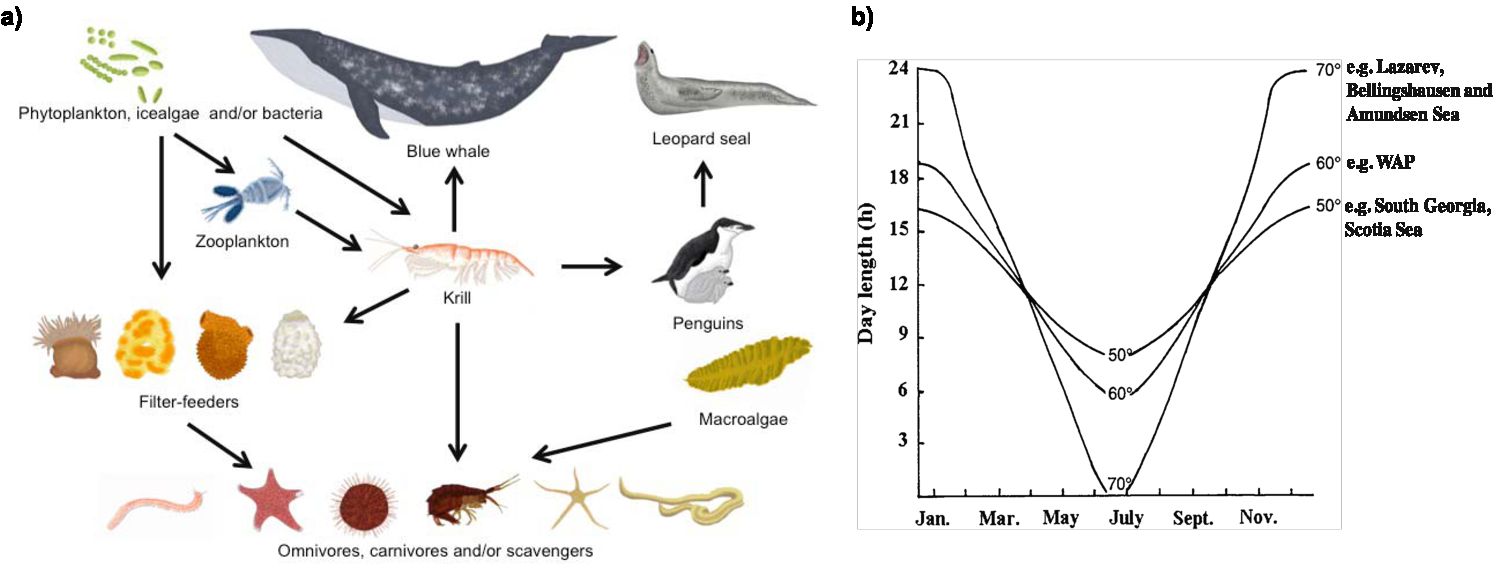
\includegraphics[width=0.85\textwidth]{../Figures/Figure1.pdf}
        \caption{a) Simplified version of the Antarctic food web by Balana
        (2013) licenced under CC BY-NC-ND 3.0 ES; b) Latitudinal light regimes
        in different regions of the Southern Ocean by \citet{meyer_performance_2012} licenced
        under CC BY 4.0.}
        \label{figure1}
\end{figure}

Commercial interest in Antarctic krill and fishery are growing considering its
high biomass, improved harvesting techniques and the increasing demand for
newly developed krill products \citep{nicol_fishery_2012}. Antarctic krill is
considered of high nutritional value when used as 'krill meal' in aquaculture \citep{yoshitomi_effect_2007} and for the production of dietary supplements and
pharmaceutical products because of their suggested beneficial properties for
human health \citep{tou_krill_2008}. Krill fishery in the Southern Ocean is
currently managed by the Commission for the Conservation of Antarctic Marine
Living Resources (CCAMLR). However, sustainable fishery's management is largely
dependent on our current understanding of the Southern Ocean ecosystem and the
correct prediction of krill abundances under changing environmental conditions
in the future.

Climate change may pose another threat to Antarctic krill. It has been
predicted that global warming and associated changes in chlorophyll
concentration will reduce the favourable growth habitat of Antarctic krill, and
thereby its biomass in the Southern Ocean \citep{hill_potential_2013}. In the Southwest
Atlantic Sector, it has been reported that Antarctic krill densities have
declined associated with a southward shift of \textit{E. superba}'s
distribution and an increase in salp densities in that region \citep{atkinson_krill_2019}(Atkinson et al.,
2004, 2019). This shift has been explained by changes in sea ice extent
(Atkinson et al., 2004) and anomalies of the Southern Annular Mode \citep{atkinson_krill_2019}. Changes in Antarctic krill biomass have been linked to the survival
of upper-level predators such as penguins which indicates that climate change
may lead to profound changes in the Southern food web \citep{trivelpiece_variability_2011}.

Climate change effects in the Southern Ocean are especially relevant under the
match/mismatch hypothesis that describes how the seasonal timing of a predator
and the availability of its prey may affect recruitment, reproduction or
survival of the predator \citep{durant_climate_2007}. In particular, Antarctic krill
may be influenced by temporal and spatial changes in phytoplankton distribution
that do not match its seasonal requirements for recruitment or reproductive
processes. However, these effects are difficult to predict, because the
mechanisms and the flexibility of Antarctic krill's seasonal timing system are
poorly understood.

\section{Pronounced Seasonal Cycles of \textit{E. superba} in the Field}

\begin{wrapfigure}{R}{0.5\textwidth}
        \centering
        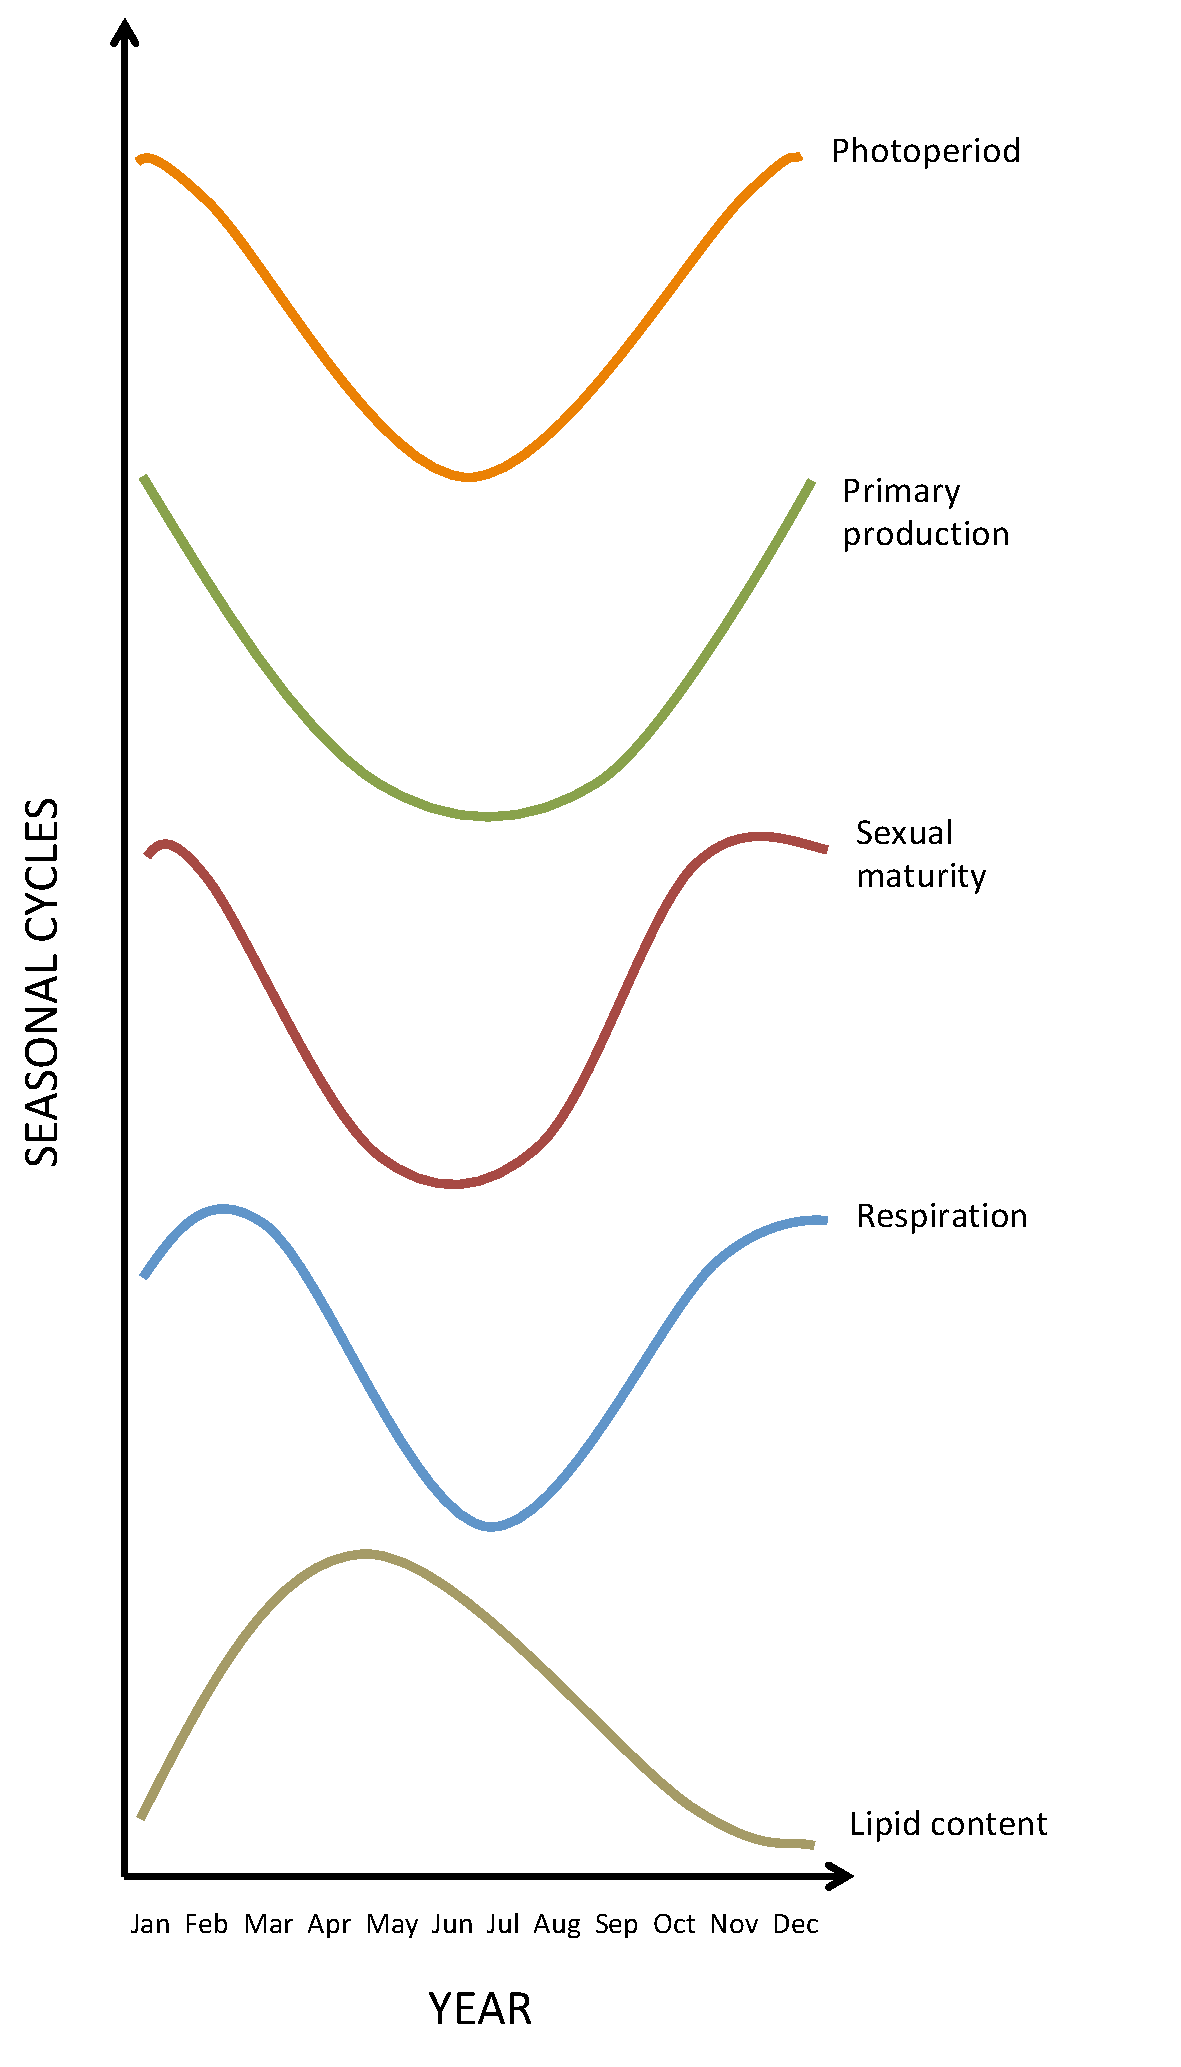
\includegraphics[height=9cm,keepaspectratio]{../Figures/Figure2.pdf}
        \caption{Schematic representation of seasonal cycles of photoperiod and
        primary production in the Southern Ocean, and sexual maturity,
        respiration and lipid content of Antarctic krill following information
        from Meyer 2012, Arrigo et al. 2008, Kawaguchi et al. 2007, and
        Hellessey et al. 2018}
        \label{figure2}
\end{wrapfigure}

Pronounced seasonal variations of growth, feeding, metabolic activity
\citep{meyer_seasonal_2010}, lipid turnover \citep{ericson_seasonal_2018,
hellessey_seasonal_2018}, reproduction \citep{siegel_krill_2012} and gene
expression \citep{seear_seasonal_2012} have been observed in Antarctic krill in
the field (Fig. \ref{figure2}). Antarctic krill has evolved different
overwintering strategies to cope with the conditions of near-constant darkness
and low food availability in some regions of the Southern Ocean
\citep{meyer_performance_2012}. The by far most important strategy is the
reduction of physiological functions consistent with a state of quiescence
observed in Antarctic krill. Respiration is severely reduced during the winter
season and may drop down to 30\% of the summer rates
\citep{meyer_seasonal_2010, quetin_behavioral_1991}. Moreover, a significantly
lower activity of the metabolic key enzymes citrate synthase
\citep{cullen_seasonal_2003, meyer_feeding_2002} and malate dehydrogenase
\citep{meyer_seasonal_2010, pape_melatonin_2008} was found in autumn and
winter. In the course of winter-metabolic depression, low feeding activity has
been observed, with indications that Antarctic krill can switch to alternative
food sources like zooplankton or ice-algae \citep{atkinson_feeding_2002,
meyer_seasonal_2010}. As a consequence, growth rates of adult krill are
extremely reduced
%FIXME: Kawaguchi 1986 is missing in the bibtex!
during winter \citep{meyer_seasonal_2010}, even shrinkage has been reported
\citep{quetin_behavioral_1991}. The seasonal accumulation of lipid stores and
their utilisation during winter promotes survival of adult krill during periods
of low food availability \citep{falkowski_global_2000, hagen_lipids_2000,
hagen_lipid_2001, meyer_seasonal_2010, quetin_behavioral_1991}. Moreover,
Antarctic krill shows a pronounced seasonal cycle of maturity which is
characterized by the regression of its external sexual traits towards winter
and the sexual re-maturation towards spring \citep{kawaguchi_male_2007}. Gene
expression analysis of seasonal Antarctic krill samples near the Antarctic
Peninsula revealed an upregulation of genes related to feeding and digestion,
respiration, motor activity, immunity and vitellogenesis in summer krill with
respect to winter \citep{seear_seasonal_2012}.

% Figure 2


Antarctic krill is able to synchronize its seasonal life cycle to local
photoperiod and food supply in the different latitudinal habitats of the
Southern Ocean. Regional differences in the timing of reproduction \citep{spiridonov_spatial_1995}, growth \citep{kawaguchi_fishing_2006}, feeding activity and lipid storage \citep{schmidt_feeding_2014}, and gene expression \citep{seear_seasonal_2012} have been
observed in the field. \citet{spiridonov_spatial_1995} investigated the spawning season of
Antarctic krill in different regions of the Southern Ocean and discussed that
the reproductive timing is largely dependent on the variation of  seasonal sea
ice cover and the timing of phytoplankton blooms. 

\citet{kawaguchi_fishing_2006} reported differences in the growth period of Antarctic
krill examining the Southwest Atlantic Sector and the Indian Ocean sector. The
authors suggested that the earlier timing of the phytoplankton bloom at lower
latitudes might advance the growth period of Antarctic krill. Differences in
the overwintering behaviour of Antarctic krill were observed by \citet{schmidt_feeding_2014} and \citet{seear_seasonal_2012} in different latitudinal habitats of the
Southern Ocean. Antarctic krill from the low-latitude region South Georgia had
higher feeding activities and lower lipid stores during winter compared to the
high-latitude region Lazarev Sea where Antarctic krill experienced
near-constant darkness and the strongest limitation in food supply \citep{schmidt_feeding_2014}. Similar differences were found on the gene expression level, where
winter Antarctic krill from South Georgia showed higher gene activities related
to feeding, digestion and immunity with respect to krill from the Antarctic
Peninsula \citep{seear_seasonal_2012}.

\section{Seasonal timing mechanisms in \textit{E. superba}}

The variable light, food, and temperature regimes may play a role in the
regulation of \textit{E. superba}'s seasonal cycles in the different latitudinal
habitats of the Southern Ocean (Fig. \ref{figure3}). Controlled laboratory experiments were
conducted to unravel the specific effects of these parameters on the different
seasonal processes in Antarctic krill. Higher water temperatures and high food
supply were found to increase the growth rates of Antarctic krill \citep{brown_temperature_2010, bucht_isolation_1991}, whereas seasonal changes of photoperiod modulated a
seasonal growth pattern \citep{piccolin_photoperiodic_2018}. \citet{kawaguchi_male_2007} found
that favourable feeding conditions accelerate the sexual maturation process of
Antarctic krill. The initiation of sexual maturation and spawning were also
observed when exposing Antarctic krill to long photoperiods \citep{hirano_antarctic_2003, teschke_effects_2008}. These long photoperiodic conditions also triggered
an enhanced lipid catabolism that was suggested to be necessary for the
maturation process \citep{teschke_effects_2008}. During long-term laboratory
experiments of constant food supply, different simulated light regimes flexibly
adjusted the seasonal cycle of maturity in Antarctic krill \citep{brown_flexible_2011}. The metabolic activity of Antarctic krill was observed to be higher
under long photoperiods similar to summer and autumn conditions compared to the
simulated winter condition 'constant darkness' \citep{teschke_simulated_2007}, while
the same study indicated that Antarctic krill might not be able to respond to
high food concentrations under constant darkness. Although food supply and
temperature have the potential to affect the respiration rates of Antarctic
krill, these factors do not change the general seasonal pattern of metabolic
activity \citep{brown_long-term_2013}. Recently, \citet{piccolin_photoperiodic_2018} confirmed in
long-term experiments that a simulated annual light regime could trigger the
seasonal cycle of metabolic activity in Antarctic krill. These seasonal
photoperiodic effects on krill's metabolic cycle were also found on gene
expression level \citep{piccolin_photoperiodic_2018, seear_effects_2009}.

% Figure 3

\begin{figure}
        \centering
        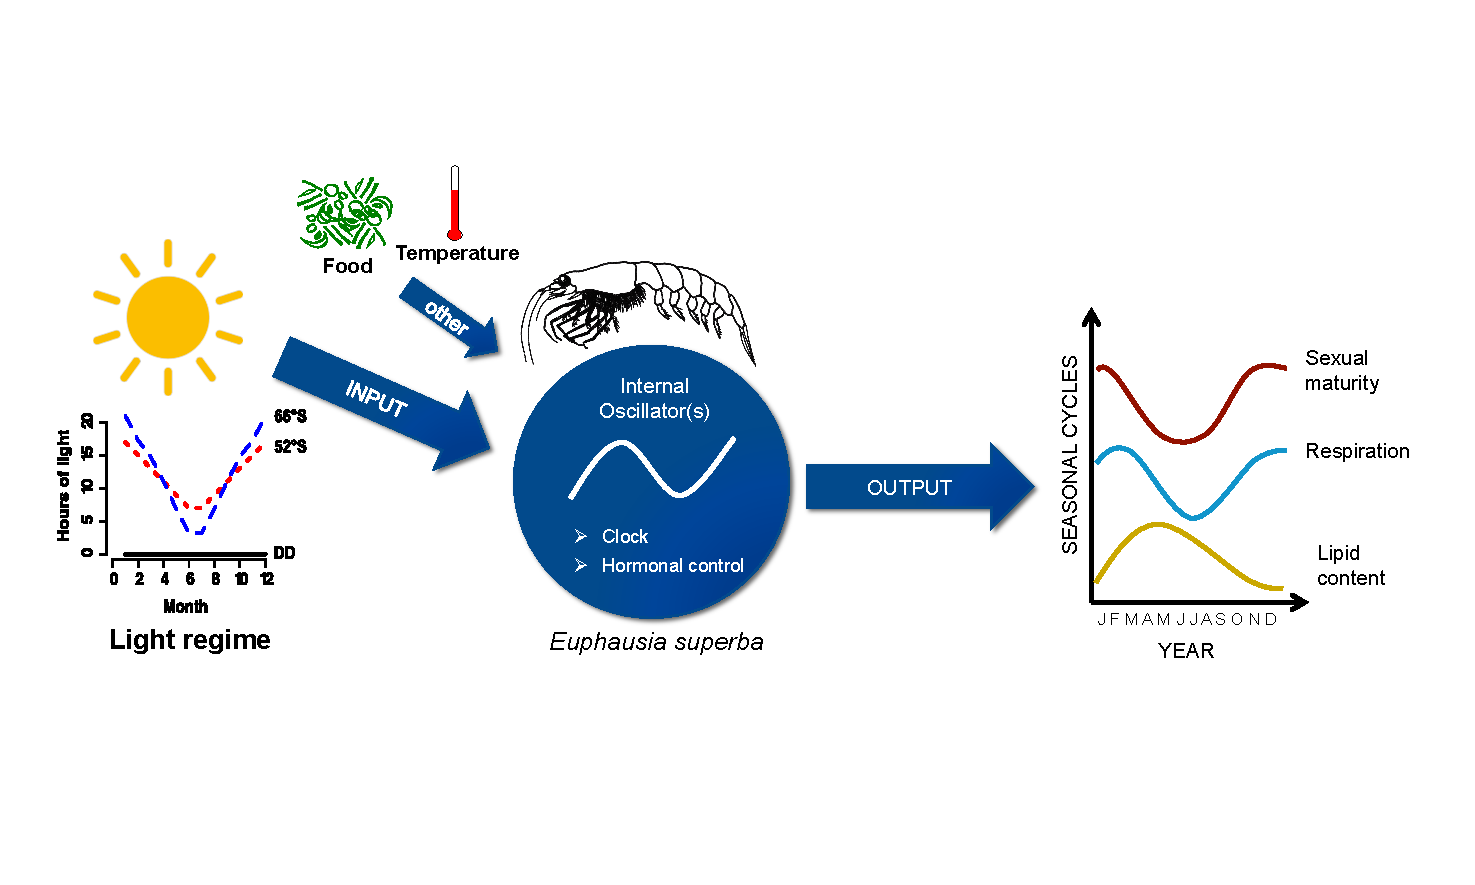
\includegraphics[width=0.85\textwidth]{../Figures/Figure3.pdf}
        \caption{Schematic representation of the seasonal timing system of Antarctic krill.}
        \label{figure3}
\end{figure}

These studies reveal that light regime and seasonal changes in photoperiod are
major cues that entrain the seasonal rhythms of growth, maturity, metabolic
activity and gene expression in Antarctic krill. It has been suggested that
these seasonal rhythms are controlled by an endogenous timing system with
photoperiod as timing cue (zeitgeber) \citep{brown_flexible_2011, brown_long-term_2013, piccolin_photoperiodic_2018}. An endogenous timing system (circannual clock) is characterized by
the observation that seasonally rhythmic patterns persist, even if the actual
zeitgeber is not present \citep{visser_phenology_2010}. Such evidence was found in
Antarctic krill during long-term laboratory experiments where seasonal patterns
of maturity, growth and metabolic activity were observed under constant
darkness \citep{brown_flexible_2011, piccolin_photoperiodic_2018}.

In general, the molecular mechanisms of seasonal timing systems are poorly
understood, but there are indications that the circadian (daily) clock may play
role for photoperiodic time measurement and consequently the timing of seasonal
life cycle events \citep{helm_annual_2013}. In eukaryotes, the circadian clock
functions as an approximately 24-h oscillator via interlaced
transcriptional/posttranslational feedback loops that are synchronized by an
environmental factor such as photoperiod \citep{mackey_biological_2007}. In insects, circadian
clock genes were found to play an important role for the seasonal photoperiodic
timing of diapause (review by \citet{goto_roles_2013, meuti_evolutionary_2013, meuti_functional_2015}, with exceptions (e.g. \citet{emerson_evolution_2009})). The investigation of
latitudinal clines of photoperiodism showed that insect populations generally
showed higher critical photoperiods for the initiation of diapause at higher
latitudes, and latitudinal adaptation of their photoperiodic response has been
linked to clock gene polymorphisms \citep{hut_latitudinal_2013}. Photoperiodic plasticity
may also be based on the differential expression of clock genes \citep{hodkova_period_2003} depending on season and latitude. Moreover, it is speculated, if
non-coding RNA or epigenetic modifications play a role in the regulation of
%missing reference in bibtex helm and stevenson 2014
circannual rhythms (Helm and Stevenson, 2014).

In Antarctic krill, molecular studies have analysed the functioning of its
visual perception system and its circadian clock \citep{biscontin_opsin_2016, biscontin_functional_2017}. Different opsin genes were identified in Antarctic krill that are
important for the visual perception of light of different wavelengths
\citep{biscontin_opsin_2016}. The circadian clock machinery of Antarctic krill was
characterized by \citet{biscontin_functional_2017} who found that the core clock
resembled both insect's and mammalian circadian clock systems with a light
mediated degradation mechanism that suggested light as the main zeitgeber.
Controlled laboratory experiments revealed that the daily oscillations of clock
genes in Antarctic krill varied under variable seasonal conditions of
photoperiod and became arrhythmic under mid-winter and mid-summer conditions
\citep{piccolin_seasonal_2018}. Antarctic krill's circadian clock has not only been
linked to the timing of daily rhythms of metabolic activity \citep{de_pitta_antarctic_2013, piccolin_seasonal_2018, teschke_circadian_2011} and diel vertical migration \citep{gaten_is_2008}, but it is also suggested to play a role for the seasonal
day length measurement and the regulation of seasonal rhythms in Antarctic
krill based on the observation of seasonal patterns of clock gene expression in
Antarctic krill \citep{piccolin_photoperiodic_2018}.

In crustaceans, circadian pacemakers (clocks) are located in the nervous
system, in particular in retina of the eye, the eyestalk, the brain and the
caudal photoreceptor \citep{arechiga_distributed_2002, rodriguez_y_baena_could_2008} and may be linked to neuroendocrine control of seasonal rhythms. Seasonal
life cycle events in decapods are mediated by various neuropeptides and
signalling molecules that originate from the X-organ-sinus gland system of the
eyestalk ganglia, brain, the thoracic ganglia, the Y-organ and the mandibular
organ \citep{nagaraju_reproductive_2011}. Important hormones comprise the 'CHH-superfamily'
including the crustacean hyperglycaemic hormone, the moult-inhibiting hormone,
the gonad/vitellogenesis-inhibiting hormone and the mandibular organ-inhibiting
hormone that have multiple functions in carbohydrate and lipid metabolism,
reproduction, moulting, osmoregulation and the regulation of methyl farnesoate
synthesis from the mandibular organ (review by \citet{webster_chh-superfamily_2012}). Other
hormones that control moulting and reproduction in crustaceans include methyl
farnesoate \citep{reddy_metabolic_2014}, ecdysteroids and 'vertebrate-type' steroids
\citep{lafont_steroids_2007}, and prostaglandins (review by \citet{nagaraju_reproductive_2011}).

In Antarctic krill, studies on the neuroendocrine control of seasonal processes
are rare \citep{bucht_isolation_1991, pape_melatonin_2008, seear_seasonal_2012, toullec_transcriptome_2013}. \citet{bucht_isolation_1991} studied changes in hemolymph titre of
ecdysone-equivalents in the different moult stages of Antarctic krill. \citet{pape_melatonin_2008} were not able to detect melatonin in Antarctic krill and therefore
rejected the hypothesis that it played a role in regulating the seasonal
metabolic cycle of Antarctic krill \citep{teschke_simulated_2007}.  In the field,
seasonal gene expression patterns of the neuropeptide neuroparsin and
insulin-like peptides have been discussed in relation to the seasonal
reproductive physiology of Antarctic krill \citep{seear_seasonal_2012}. In the ice
krill, \textit{Euphausia crystallorophias}, various neuropeptide hormones were
identified including members of the CHH superfamily \citep{toullec_transcriptome_2013}. The
recently developed transcriptome database may provide a source for \textit{E.
superba}-specific target sequences of neuropeptides \citep{sales_krilldb:_2017}.

\section{Research objectives}
The current environmental changes in the Southern Ocean and the increasing
commercial interest in Antarctic krill emphasise the need to better understand
the adaptability of \textit{E. superba} in different latitudinal regions of the
Southern Ocean, especially under the aspect of potential mismatches in
biological timing. It has not yet been investigated, if different latitudinal
light regimes regulate the flexible seasonal physiology and behaviour of
Antarctic krill in its diverse latitudinal habitats.  In general, the seasonal
timing system of Antarctic krill is not well understood including the potential
involvement of the circadian clock and the neuroendocrine control of seasonal
rhythms in Antarctic krill. Laboratory experiments that observe the seasonal
cycle of Antarctic krill under controlled photoperiodic conditions over a
period of multiple years and simulating different latitudinal light regimes are
still lacking.

This dissertation aimed to understand the role of different latitudinal light
regimes on the seasonal cycle of Antarctic krill focussing on (a) the molecular
characterization of seasonal rhythms in different latitudinal habitats in the
field (Publication 1), and (b) the investigation of seasonal rhythms under a
two-year photoperiodic-controlled laboratory experiment with constant food
supply (Publication 2 \& 3). The following research objectives were addressed
in the three different chapters of the dissertation:

\begin{enumerate}
\item Investigation of seasonal and regional differences in gene expression of
        summer and winter Antarctic krill from three different latitudinal
                regions: South Georgia (\SI{54}{\degree}S), South
                Orkneys/Bransfield Strait (\SI{60}{\degree}S-\SI{63}{\degree}S)
                and Lazarev Sea (\SI{62}{\degree}S-\SI{66}{\degree}S)
                (Publication 1)
\item Analysis of seasonal cycles of growth, feeding, lipid metabolism and
        maturity of Antarctic krill under the simulated light regimes
                \SI{52}{\degree}S, \SI{66}{\degree}S, and constant darkness
                (Publication 2)
\item Characterization of seasonal expression patterns of genes involved in
        different metabolic processes, seasonal timing, reproduction, feeding
                and development under the simulated light regimes
                \SI{52}{\degree}S, \SI{66}{\degree}S, and constant darkness
                (Publication 3)
\end{enumerate}

A range of different methods were implemented to investigate the effect of
latitudinal light regime on Antarctic krill. An RNAseq approach was used to
characterize the seasonal and latitudinal gene expression differences in
Antarctic krill in the field and to identify suitable seasonal target genes
with focus on genes with potential regulatory functions in the seasonal cycle
of Antarctic krill. For the first time, a two-year laboratory experiment was
conducted that simulated different latitudinal light regimes and constant food
supply. Antarctic krill from the laboratory experiments was investigated using
morphometric and lipid content analysis, and gene expression data from custom
designed TaqMan cards.

The findings of this dissertation improve our understanding of the effect of
different latitudinal light regimes on seasonal cycles in Antarctic krill and
their underlying molecular mechanisms.

\printbibliography[heading=subbibliography]
